\documentclass[a4paper]{report}
\author{Jure Kos}
\title{Vaja 62, Modeli optičnih naprav}
\date{5.5.2022}
\usepackage{graphicx}
\graphicspath{ {./images/} }
\begin{document}

\maketitle

\chapter*{Uvod}
\section*{Projekcijki aparat}
Slika prikazuje poenostavljeno shemo projekcijskega aparata. Sestavljen je iz svetila, kondenzorja in objektiva. Predmet, ki ga projiciramo pa je film ali diapozitiv, ki stoji tik za kondenzorjem. Naloga kondenzorja je, da preslika svetilo v sredino objektiva. Skoraj vsa svetloba, ki pada na kondenzor in gre za tem skozi predmet, pride tako na zaslon. Slika je zato enakomerno osvetljena in, ker preslikavamo le s sredine objektiva, tudi manj popačena. Objektiv naravnamo tako, da je slika na zaslonu ostra. Ker je zaslon običajno precej oddaljen je pri tem predmet malo pred goriščno ravnino objektiva. Povečavo projekcijskega aparata definiramo s kvocientom velikosti in slike:

\[N=\frac{y'}{y}=\frac{x'+f}{x+f}\]

\begin{figure}[htp]
    \centering
    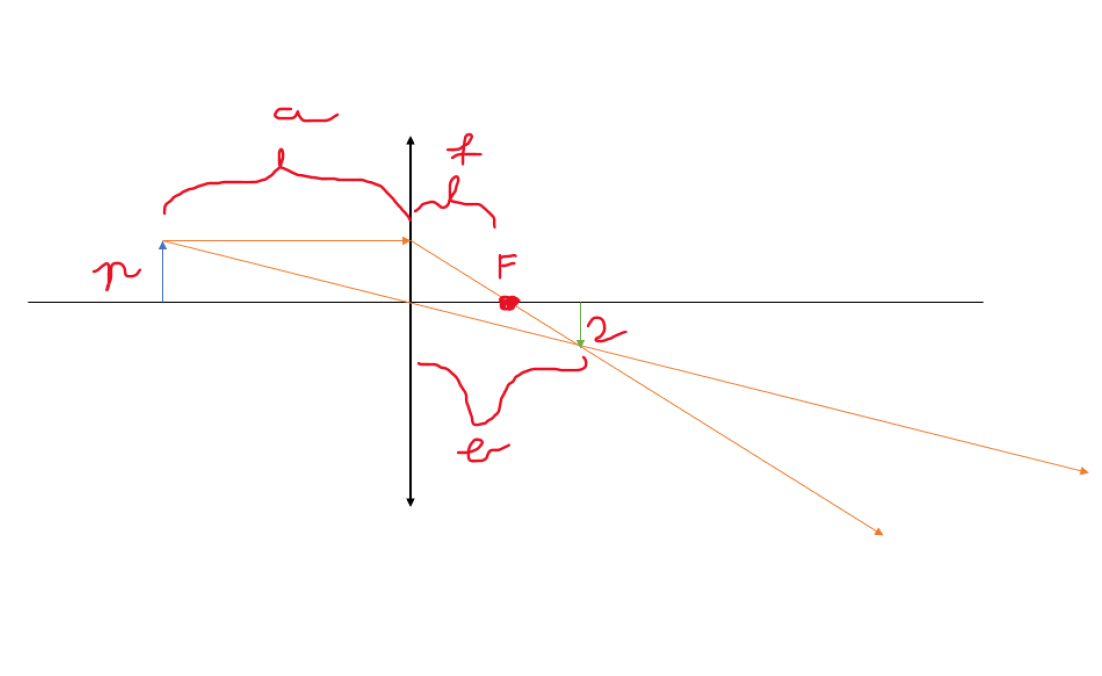
\includegraphics[width=\textwidth]{Projektor.png}

\end{figure}

\section*{Daljnogled}
Oddaljene predmete slabo ali sploh ne ločimo s prostimi očmi, ker jih gledamo s premajhnimi zornimi koti. Z daljnogledom te zorne kote povečamo. Naravno je torej, da definiramo povečavo daljnogleda kot razmerje zornega kota, pod katerim vidimo oddaljen predmet skozi daljnogled, in kota, s katerim ga vidimo s prostimi očmi. Zaradi lažjega računanja pa mnogi definirajo povečavo daljnogleda kot razmerje tangensov omenjenih kotov. Dokler so zorni
koti majhni, sta obe definiciji ekvivalentni.

\begin{figure}[htp]
    \centering
    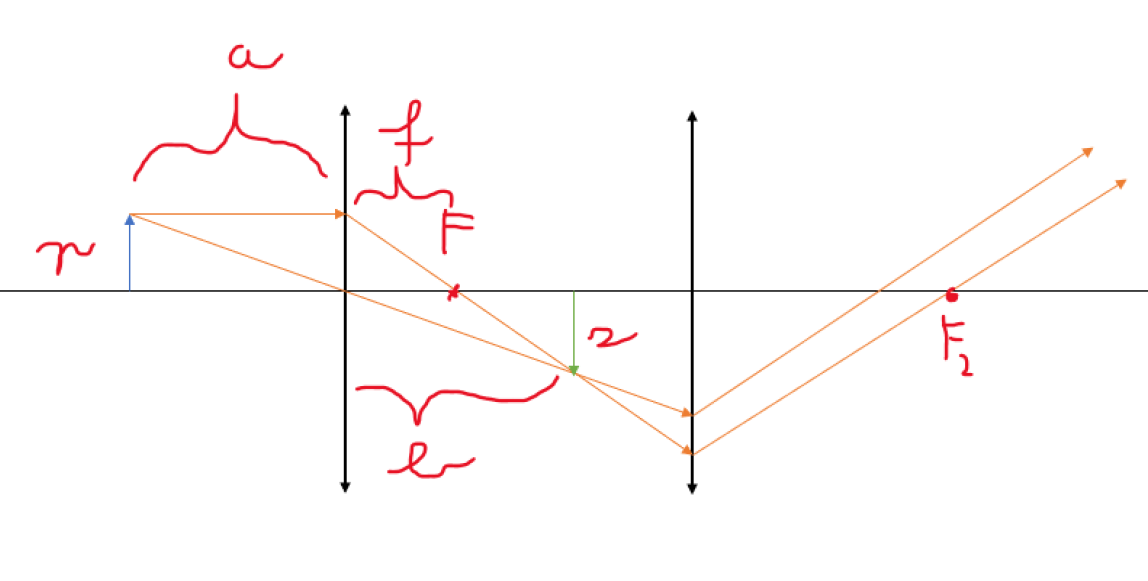
\includegraphics[width=\textwidth]{Daljnogled.png}

\end{figure}

\noindent Preprost model daljnogleda je sestavljen iz dveh leč. Leča, ki je obrnjena proti predmetu, je vedno zbiralna in jo imenujemo objektiv. Ta preslika opazovani predmet malo za svojo goriščno ravnino. Dobljeno realno sliko gledamo skozi drugo lečo, ki jo imenujemo okular. Okular je lahko zbiralna ali pa razpršilna leča. Ponavadi uporabljamo kot okular zbiralno lečo, ker dobimo z razpršilno lečo majhno vidno polje. Okular postavimo najraje tako, da se njegova goriščna ravnina krije z ravnino slike, ki jo da objektiv. Tako vidimo skozi okular navidezno sliko v neskončnosti. Slika kaže, da je povečava daljnogleda v tem primeru enaka:  

\[N=\frac{tan\phi'}{tan\phi}=\frac{f_1}{f_2}\cdot \frac{1}{1-\frac{f_1}{a}}\]

Kjer je $f_1$ goriščna razdalja objektiva, $f_2$ goriščna razdalja okularja, a pa je oddaljenost predmeta od objektiva. Vidimo da mora biti $f_1 > f_2$, običajno pa
je $a \gg f_1$. Objektiv tedaj preslika predmet skoraj v goriščno ravnino; gorišči
obeh leč se približno prekrijeta.

\section*{Mikroskop}
Mikroskop služi za opazovanje majhnih predmetov, ki bi jih sicer niti v normalnih zornih kotin ne mogli razlošiti. Kakor daljnogled, tudi mikroskop poveša zorni kot opazovanega predmeta. Mikroskop sestavljata objektiv in okular. Oba sta konveksni leši z majhnima goriščnima razdaljama. Predmet je nekaj pred sprednjo goriščno ravnino objektiva, tako da nastane na notranji strani realna povešana slika predmeta. To sliko gledamo skozi okular, ki deluje kot lupa. Povešavo definiramo kot razmerje tangensa kota, s katerim vidimo predmet skozi mikroskop in tangensa kota, s katerim bi ga videli s prostimi ošmi v normalni
zorni razdalji (r = 25cm).

\[N=\frac{tan\phi_1}{tan\phi_2}=\frac{dr}{f_1f_2}\]

kjer je d razdalja med notranjima goriščema leč, $f_1$ goriščna razdalja med objektivoma
in $f_2$ goriščna razdalja okularja. Izraz je produkt povečave objektiva:

\[N_1=\frac{d}{f_1}=\frac{Y}{y}\]

\begin{figure}[htp]
    \centering
    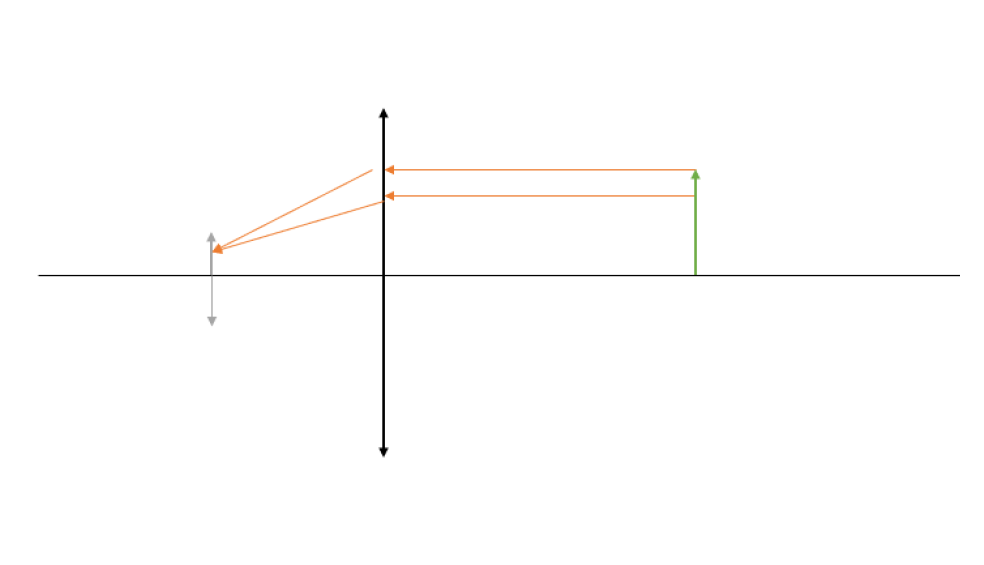
\includegraphics[width=\textwidth]{Mikroskop.png}

\end{figure}

\chapter*{Naloga}
1. Sestavi projekcijski aparat, projiciraj na zaslon diapozitiv in določi povečavo.\\
2. Sestavi daljnogled in mu določi povečavo.\\
3. Sestavi mikroskop in mu določi povečavo.



\chapter*{Meritve}


Meritve projekcijskega aparata:

\begin{center}
    \begin{tabular}{|c|c|} 
      \hline
      Ocenjena goriščna razdalja objektiva & 33mm $\pm$ 5mm \\
      \hline
      Ocenjena goriščna razdalja objektiva & 11mm $\pm$ 5mm \\
      \hline
      razdalja med sliko in objektivom & 256mm $\pm$ 5mm 0\\
      \hline
      višina slike & 33mm $\pm$ 220mm \\
      \hline
      višina predmeta v projekciji & 232mm $\pm$ 5mm \\
      \hline
      goriščna razdalja objektiva & 110mm $\pm$ 5mm \\
      \hline

    \end{tabular}
  \end{center}
  
  
\noindent  Meritve daljnogleda:

  \begin{center}
    \begin{tabular}{|c|c|} 
      \hline
      Goriščna razdalja okularja & 134mm $\pm$ 5mm \\
      \hline
      Goriščna razdalja objektiva & 58mm $\pm$ 5mm \\
      \hline
      Razdalja med objektivom in okularjem & 570mm $\pm$ 5mm 0\\
      \hline
      Ocenjena povečava & 3 \\
      \hline
      Dolžina sobe & 13m $\pm$ 20cm \\
      \hline
      

    \end{tabular}
  \end{center}
  
  
\noindent Meritve mikroskopa: 
 
  \begin{center}
    \begin{tabular}{|c|c|} 
      \hline
      Goriščna razdalja okularja & 58m $\pm$ 5mm \\
      \hline
      Goriščna razdalja objektiva & 87mm $\pm$ 5mm \\
      \hline
      Razdalja med objektivom in okularjem & 300mm $\pm$ 5mm 0\\
      \hline
      Ocenjena povečava & 6 \\
      \hline

    \end{tabular}
  \end{center}
  
  
  \chapter*{Računi}
  1. Projektor:\\
  Po enačbi $N=\frac{y'}{y}$ dobimo
  
  \[N=1,05 \pm 0,1\]
  
  \noindent 2. Daljnogled:\\
  Po enačbi $N=\frac{f_1}{f_2}\cdot \frac{1}{1-\frac{f_1}{a}}$ dobimo
  
  \[N=2,3 \pm 0,2\]
  
  \noindent 3. Mikroskop:\\
  Po enačbi $N=\frac{dr}{f_1f_2}$ dobimo
  
  \[N=14\pm1\]
\end{document}